\section{PHÁT HÀNH ỨNG DỤNG}
Đầu tiên để phát hành ứng dụng, cần phải tải thư viện eas-cli để có thể phát hành ứng dụng 
\begin{figure}[H]
    \centering
    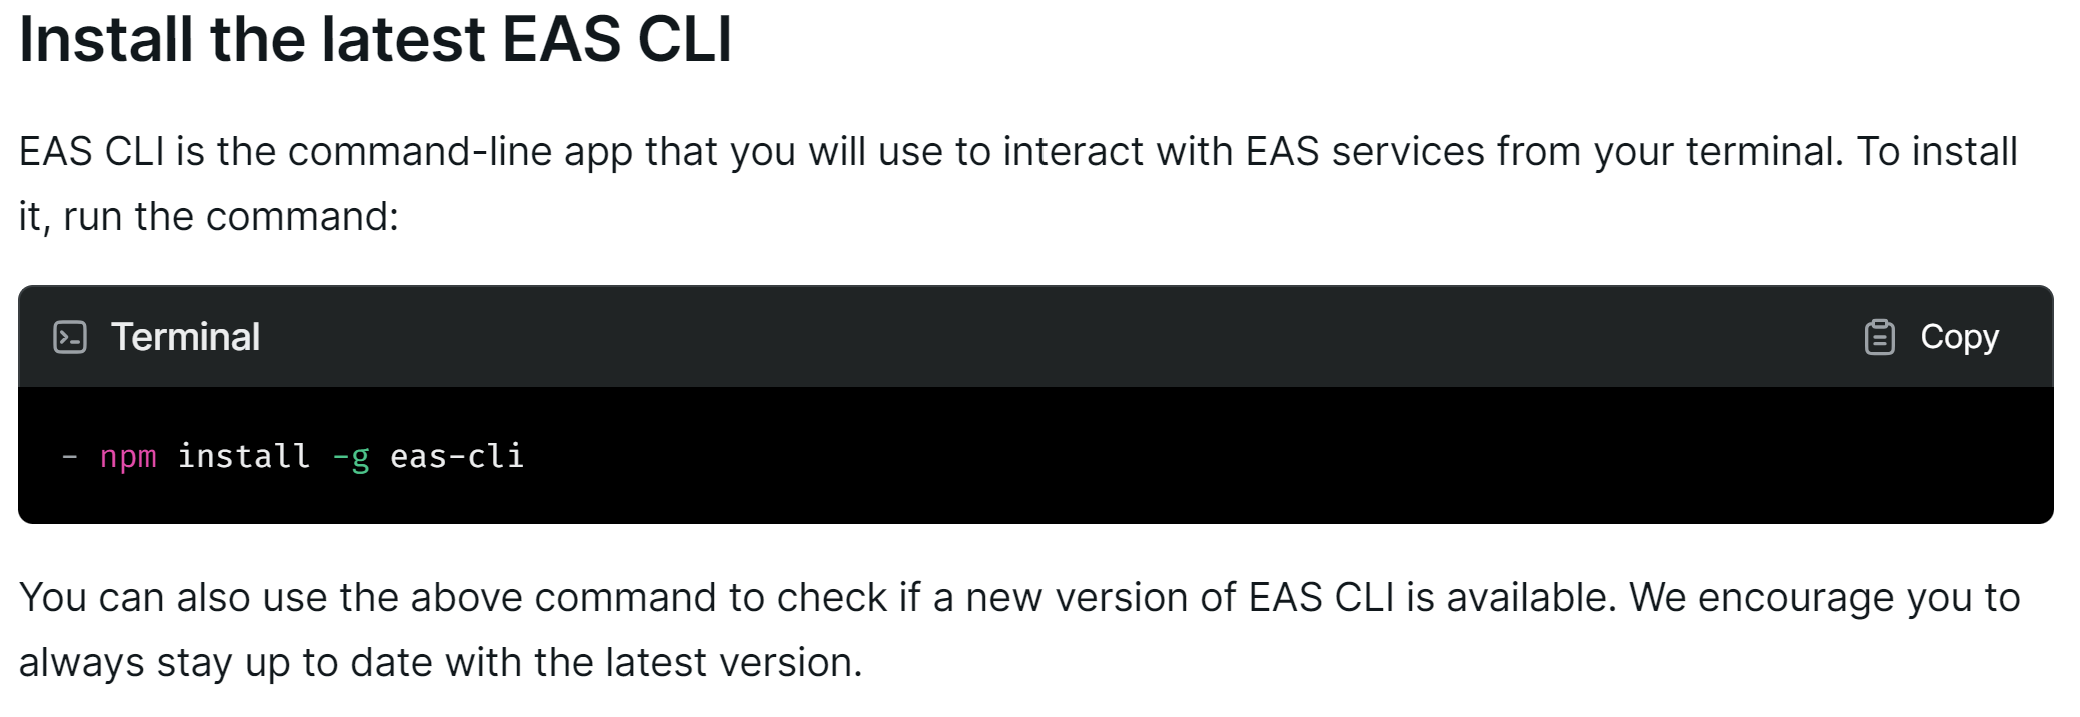
\includegraphics[width=1\textwidth]{Images/Build_app/eas_install.png}
    \caption{Tải thư viện eas-cli}
\end{figure}
Ở dự án này sử dụng expo go để phát triển do đó cần phải đăng nhập vào tài khoản để kích hoạt
\begin{figure}[H]
    \centering
    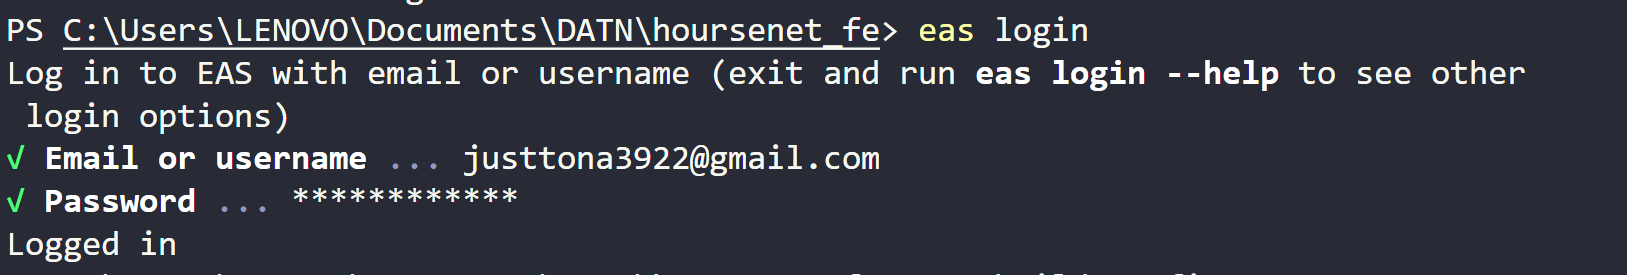
\includegraphics[width=1\textwidth]{Images/Build_app/build_login.png}
    \caption{Đăng nhập tài khoản expo}
\end{figure}
Sau đó sẽ tiến hành cấu hình file eas-json, ở đây để phát hành dưới dạng file .apk , nên buildType sẽ ở dạng .apk, chọn cli với version phù hợp
\begin{figure}[H]
    \centering
    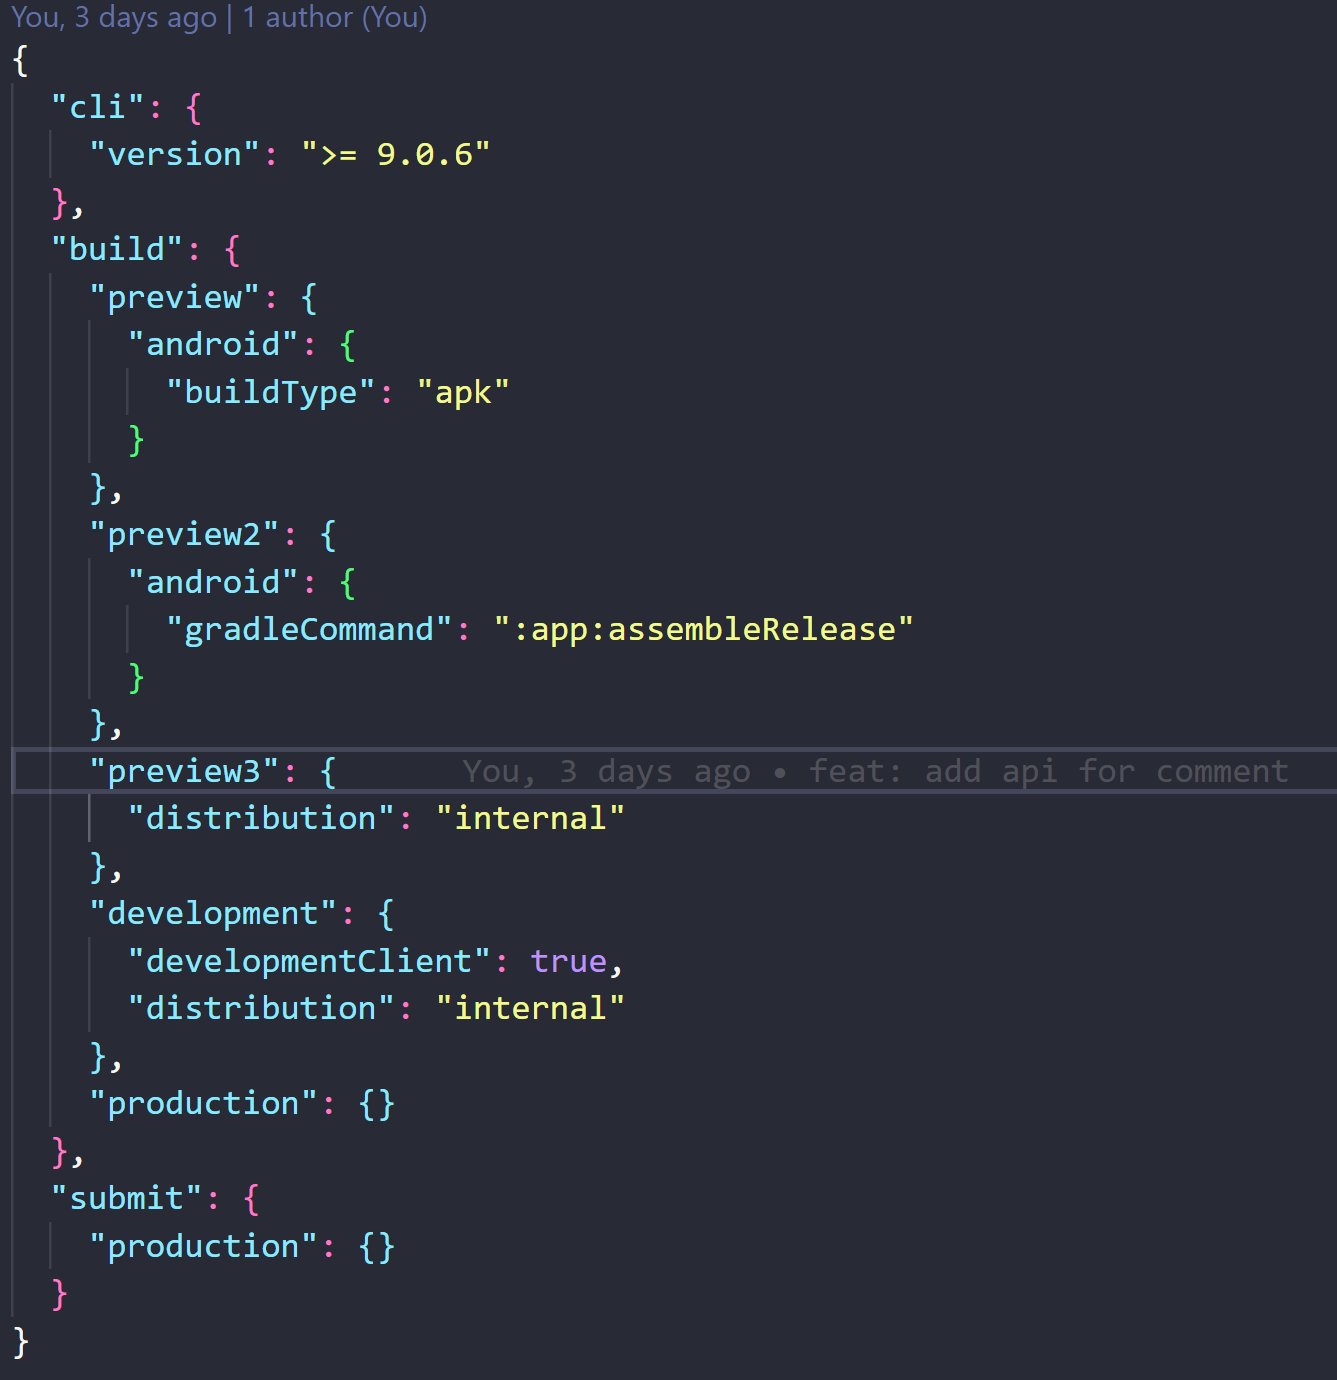
\includegraphics[width=1\textwidth]{Images/Build_app/eas-json.png}
    \caption{Cấu hình file eas-json}
\end{figure}
Nhập lệnh \textbf{eas build:configure} để xây dựng app dựa trên cấu hình file eas-json đã thiết lập ở phía trên
\begin{figure}[H]
    \centering
    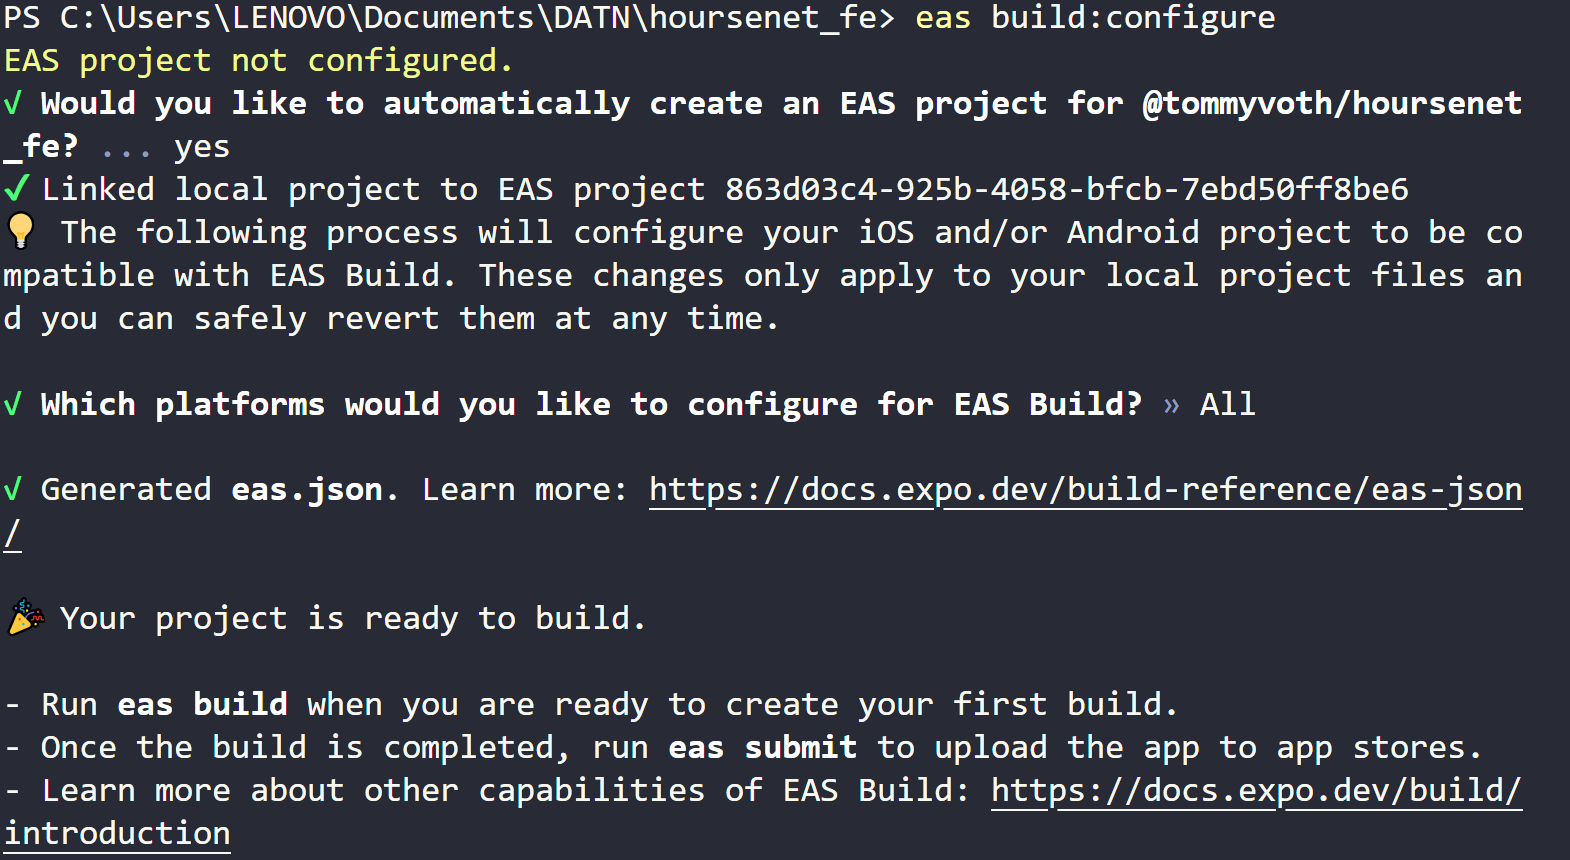
\includegraphics[width=1\textwidth]{Images/Build_app/build_configure.png}
    \caption{Xây dựng cấu hình cho app}
\end{figure}
Nhập lệnh \textbf{eas build -p android --profile preview} để xây dựng và phát hành ứng dụng trên hệ điều hành android dưới dạng file .apk
\begin{figure}[H]
    \centering
    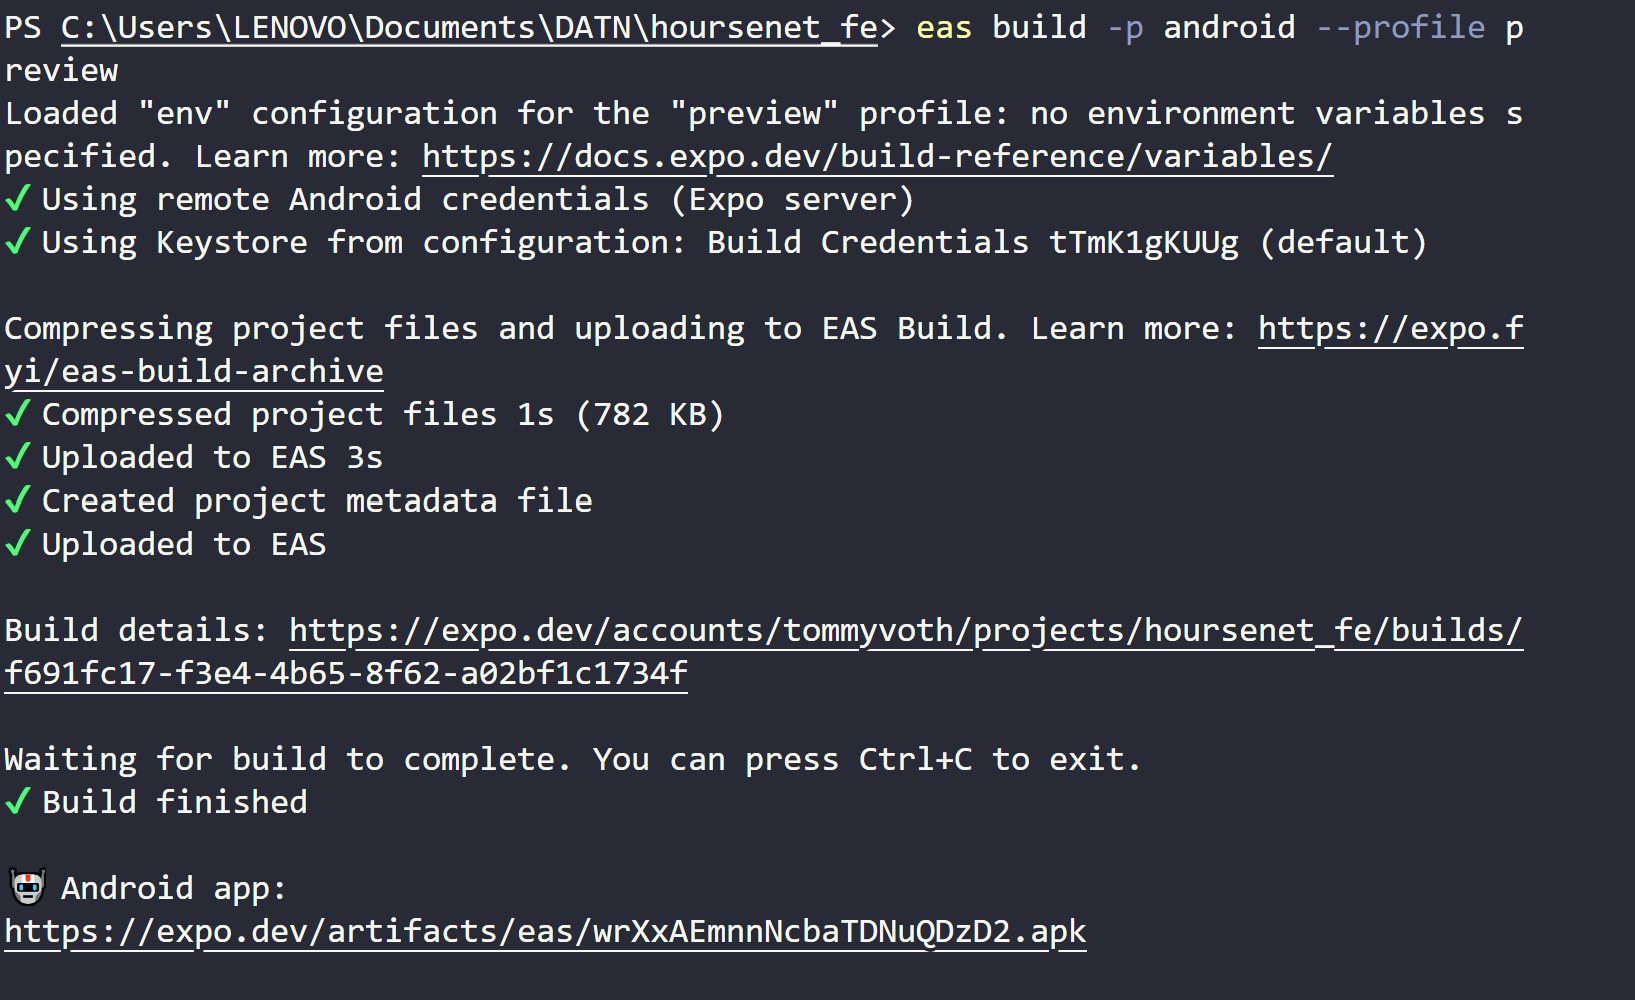
\includegraphics[width=1\textwidth]{Images/Build_app/build_android.png}
    \caption{Xây dựng ứng dụng cho hệ điều hành android}
\end{figure}